%==============================================================================
%  Computer Systems Security (SSC), 2026-27 -- Universidade do Minho
%  Lab report 1 (deliverable): Block 1 -- Lab 1 (First Contact) + Lab 2 (Threat Modelling)
%  Sources: Labs 1 + 2. Build: pdflatex report1.tex (images/ + lab notes)
%==============================================================================
\documentclass[a4paper,11pt]{article}

%------------------------------------------------------------ codificacao e fontes
\usepackage[utf8]{inputenc}
\usepackage[T1]{fontenc}
\usepackage[portuguese]{babel}
\usepackage{textcomp}
\usepackage{lmodern}
\usepackage{tgheros}                 % sans-serif usado nos titulos (TeX Gyre Heros)
\usepackage{microtype}

%------------------------------------------------------------ geometria da pagina
\usepackage[margin=2.5cm,headheight=15pt,footskip=32pt]{geometry}

%------------------------------------------------------------ palete de cores
\usepackage[table]{xcolor}
\definecolor{sscnblue}{RGB}{15,42,79}      % titulos, capa
\definecolor{sscblue}{RGB}{31,92,156}      % acentos, links, subtitulos
\definecolor{sscline}{RGB}{198,207,219}    % filetes e molduras
\definecolor{sscbg}{RGB}{245,247,250}      % fundos claros
\definecolor{sscmute}{RGB}{95,104,116}     % texto secundario

%------------------------------------------------------------ estrutura, listas, flutuantes
\usepackage{tikz}
\usepackage{graphicx}
\usepackage{array}
\usepackage{tabularx}
\usepackage{booktabs}
\usepackage{float}
\usepackage{caption}
\usepackage{enumitem}
\usepackage{titlesec}
\usepackage{tocloft}
\usepackage{fancyhdr}
\usepackage{listings}
\usepackage{tcolorbox}
\tcbuselibrary{breakable}
\usepackage{hyperref}
\usepackage{lastpage}
\emergencystretch=2em
\hypersetup{
  colorlinks=true,
  linkcolor=sscnblue,
  urlcolor=sscblue,
  citecolor=sscnblue,
  pdftitle={Lab report 1: Block 1 (Labs 1+2) --- Threat Model},
  pdfauthor={Hugo Soares a107293},
  pdfsubject={Seguran\c{c}a de Sistemas da Computa\c{c}\~{a}o (SSC) --- Lab 1 inventory + Lab 2 threat model: DFD, STRIDE, attack tree},
  pdfkeywords={modelacao de ameacas, DFD, STRIDE, arvore de ataque, ativos, priorizacao},
  pdflang={pt}
}

\graphicspath{{images/}}

%------------------------------------------------------------ espacamento de paragrafos e listas
\setlength{\parindent}{0pt}
\setlength{\parskip}{5pt plus 1pt}
\setlist{topsep=3pt,itemsep=2pt,parsep=0pt,leftmargin=1.6em}
\setlist[itemize]{label=\textcolor{sscblue}{\textbullet}}
\setlist[enumerate]{label=\textcolor{sscnblue}{\arabic*.},ref=\arabic*}

%------------------------------------------------------------ titulos
\titleformat{\section}
  {\Large\bfseries\color{sscnblue}}{\thesection}{0.9em}{}
  [\vspace{3pt}{\color{sscline}\titlerule[0.7pt]}]
\titleformat{\subsection}
  {\large\bfseries\color{sscblue}}{\thesubsection}{0.9em}{}
\titleformat{\subsubsection}
  {\normalsize\bfseries\color{sscmute}}{\thesubsubsection}{0.9em}{}
\titlespacing*{\section}{0pt}{20pt}{10pt}
\titlespacing*{\subsection}{0pt}{15pt}{6pt}
\titlespacing*{\subsubsection}{0pt}{12pt}{4pt}

%------------------------------------------------------------ indice
\setcounter{tocdepth}{2}
\renewcommand{\cftsecfont}{\bfseries\color{sscnblue}}
\renewcommand{\cftsecpagefont}{\bfseries\color{sscnblue}}
\renewcommand{\cftsubsecfont}{\small\color{sscblue}}
\renewcommand{\cftsubsecpagefont}{\small\color{sscblue}}
\renewcommand{\cftdotsep}{1.6}
\setlength{\cftbeforesecskip}{5pt}
\setlength{\cftbeforesubsecskip}{1pt}

%------------------------------------------------------------ legendas
\captionsetup{font=small,labelfont={bf,color=sscnblue},labelsep=quad}
\captionsetup[table]{position=top}
\captionsetup[figure]{position=bottom}

%------------------------------------------------------------ cabecalho e rodape
\pagestyle{fancy}
\fancyhf{}
\fancyhead[L]{\footnotesize\color{sscmute}Laborat\'{o}rio 2 --- Modela\c{c}\~{a}o de Amea\c{c}as na Pr\'{a}tica}
\fancyhead[R]{\footnotesize\color{sscmute}\textit{Computer Systems Security (SSC)}}
\fancyfoot[C]{\footnotesize\color{sscmute}\thepage\ / \pageref{LastPage}}
\renewcommand{\headrulewidth}{0.4pt}
\renewcommand{\headrule}{{\color{sscline}\hrule width\headwidth height 0.4pt}}
\renewcommand{\footrulewidth}{0pt}

%------------------------------------------------------------ caixas de destaque
\newtcolorbox{callout}[2][]{%
  breakable, colback=sscbg, colframe=sscnblue, coltitle=white,
  fonttitle=\bfseries\small, title={#2},
  boxrule=0.6pt, arc=2pt, left=7pt, right=7pt, top=4pt, bottom=4pt,
  before skip=8pt, after skip=8pt, #1}

\newtcolorbox{note}[1][]{%
  breakable, colback=white, colframe=sscline,
  boxrule=0pt, leftrule=3pt, arc=0pt, left=8pt, right=8pt, top=4pt, bottom=4pt,
  before skip=8pt, after skip=8pt, #1}

%------------------------------------------------------------ respostas (1a., 1b., ...)
\newenvironment{answer}[1]{%
  \par\addvspace{7pt}\noindent
  \hangindent=2.4em\hangafter=1
  {\color{sscnblue}\bfseries #1\hspace{0.55em}}\ignorespaces}
  {\par\addvspace{5pt}}

%------------------------------------------------------------ listagens de terminal
\lstdefinestyle{ssc}{
  basicstyle=\ttfamily\small,
  keywordstyle=\color{sscblue}\bfseries,
  commentstyle=\color{sscmute}\itshape,
  stringstyle=\color{sscnblue},
  backgroundcolor=\color{sscbg},
  frame=single, framerule=0.4pt, rulecolor=\color{sscline},
  xleftmargin=1em, xrightmargin=1em,
  aboveskip=9pt, belowskip=9pt,
  columns=fullflexible, keepspaces=true, showstringspaces=false,
  breaklines=true, tabsize=2, upquote=true,
  literate={'}{{\textquotesingle}}1 {`}{{\textquotesingle}}1
}
\lstset{style=ssc}
\newcommand{\cmd}[1]{\textcolor{sscnblue}{\texttt{#1}}}

%------------------------------------------------------------ estilos do DFD e da arvore
\tikzset{
  ent/.style={draw=sscnblue, fill=sscbg, rounded corners=2pt, align=center,
              minimum width=3.4cm, minimum height=1.3cm, inner sep=4pt},
  proc/.style={draw=sscblue, fill=white, circle, align=center, inner sep=2pt,
               minimum size=2.6cm},
  store/.style={draw=sscnblue, fill=sscbg, align=center, inner sep=4pt,
                minimum width=3.4cm, minimum height=1.0cm},
  dflow/.style={->, >=stealth, thick, draw=sscmute, dashed},
  flow/.style={->, >=stealth, thick, draw=sscmute},
  bd/.style={draw=sscline, dashed, thick},
  flbl/.style={font=\scriptsize\itshape, text=sscmute, align=left},
  goal/.style={draw=sscnblue, fill=sscbg, rounded corners=2pt, align=center,
               text width=3.3cm, font=\scriptsize, inner sep=4pt},
  branch/.style={draw=sscblue, fill=sscbg, rounded corners=2pt, align=center,
                 text width=3.3cm, font=\scriptsize, inner sep=4pt},
  leaf/.style={draw=sscblue, fill=white, align=center, text width=2.7cm,
               font=\scriptsize\ttfamily, inner sep=3pt, minimum height=1.6cm},
  tedge/.style={draw=sscmute, thick, ->, >=stealth}
}

%------------------------------------------------------------ metadados
\title{Laborat\'{o}rio 2: Modela\c{c}\~{a}o de Amea\c{c}as na Pr\'{a}tica}
\author{Hugo Soares a107293}
\date{\today}

\begin{document}

%==============================================================================
\begin{titlepage}
\thispagestyle{empty}
\begin{center}
    \vspace*{1.0cm}
    {\large\color{sscmute}\MakeUppercase{Universidade do Minho}}\\[2pt]
    {\small\color{sscmute}Computer Systems Security (SSC) --- MCS, 2026--27}\\[8pt]
    {\color{sscline}\rule{0.8\textwidth}{0.8pt}}\\[2.2cm]

    {\LARGE\bfseries\color{sscnblue}Lab report 1: Respostas\\[6pt]
     Labs 1 + 2}\\[0.7cm]
    {\large\color{sscblue}Lab 1 (First Contact) + Lab 2 (Threat Modelling) --- um \'{u}nico PDF de respostas}\\[3.0cm]

    \colorbox{sscbg}{%
    \begin{minipage}{0.74\textwidth}
    \vspace{8pt}
    \renewcommand{\arraystretch}{1.35}
    \begin{tabular}{@{}>{\bfseries\color{sscnblue}}l l@{}}
        Disciplina & Computer Systems Security (SSC) \\
        Mestrado   & MCS, 2026--27 \\
        Institui\c{c}\~{a}o & Universidade do Minho \\
        Entrega & Lab report 1 (\'{u}nica entrega do bloco: cobre Labs 1 e 2) \\
        Aluno      & Hugo Soares a107293 \\
        Data       & \today \\
    \end{tabular}
    \vspace{8pt}
    \end{minipage}}

    \vfill
    {\footnotesize\color{sscmute}PDF de respostas: P1/P2 e Exerc\'icios dos Labs 1 e 2. O Lab 1 n\~ao tem relat\'orio pr\'oprio; as suas respostas v\~ao na Sec\c{c}\~ao Lab 1.}\\[2pt]
    {\footnotesize\color{sscmute}Nenhuma explora\c{c}\~{a}o foi realizada.}
\end{center}
\end{titlepage}
\setcounter{page}{2}


\tableofcontents
\newpage

%==============================================================================
\section{Lab 1 --- Respostas}
\subsection{Ex. 7 --- Invent\'ario da superf\'icie de ataque}
\begin{table}[H]
\centering
\caption{Invent\'ario da superf\'icie de ataque --- Lab 1, Exerc\'icio 7.}
\label{tab:inventario-lab1}
\footnotesize
\setlength{\tabcolsep}{5pt}
\renewcommand{\arraystretch}{1.3}
\begin{tabularx}{\textwidth}{@{}>{\raggedright\arraybackslash}p{3.1cm} >{\raggedright\arraybackslash}X >{\raggedright\arraybackslash}X >{\raggedright\arraybackslash}X >{\raggedright\arraybackslash}X@{}}
\toprule
\textbf{Item de superf\'icie} & \textbf{Dimens\~ao} & \textbf{Corre / \'e detido por} &
\textbf{Quem alcan\c{c}a ou modifica} & \textbf{Pergunta em aberto} \\
\midrule
\rowcolor{sscbg}
Servi\c{c}o na porta 8081 & Servi\c{c}o em escuta & Conta de servi\c{c}o n\~ao privilegiada (\cmd{svc-report})
      & Alcan\c{c}\'{a}vel em todas as interfaces; a conta de servi\c{c}o \'e a detentora
      & A l\'ogica do servi\c{c}o exp\~oe comportamento sens\'ivel ou dados inseguros? \\
\url{/usr/local/bin/backup-tool} & Bin\'ario privilegiado & Bin\'ario setuid detido por root
      & Qualquer utilizador local o pode invocar com privil\'egio elevado
      & Qual \'e o comportamento real do bin\'ario sob sem\^antica setuid? \\
\rowcolor{sscbg}
\url{/opt/maint/rotate.sh} & Execu\c{c}\~ao agendada & Root, via trabalho cron de 10 em 10 minutos
      & Escrita livre; qualquer utilizador local o pode modificar
      & Que a\c{c}\~ao privilegiada executa o script e como poderia ser abusada? \\
\url{/etc/report/report.conf} & Ficheiro sens\'ivel em repouso & Ficheiro detido por root
      & Leg\'ivel por todos os utilizadores da m\'aquina
      & S\~ao credenciais falsas ou reais, e quanto ganharia um ponto de apoio local? \\
\bottomrule
\end{tabularx}
\end{table}

\subsection{Prepara\c{c}\~ao do Lab 1 (P1, P2)}
\begin{answer}{Lab 1, P1.}
Corri \cmd{date; cat /etc/ssc-image-release} antes da sess\~ao. A Figura~\ref{fig:p1-app}
mostra a captura (imagem, n\~ao texto): a data prova que a m\'aquina j\'a estava ligada.
\'E a \textbf{SSC lab base image} \textbf{1.0}, \cmd{arch: arm64} --- VM \textbf{ARM64}
em host Apple Silicon via QEMU, cgroup v2 v\'alido.
\end{answer}

\begin{figure}[H]
\centering
\begin{tcolorbox}[colback=white,colframe=sscline,width=0.90\textwidth,
                   boxrule=0.5pt,arc=2pt,left=6pt,right=6pt,top=6pt,bottom=6pt]
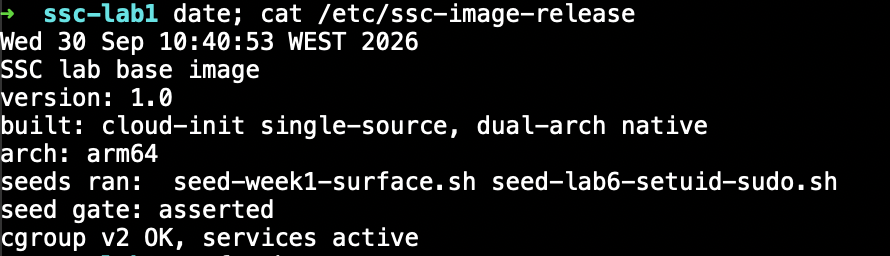
\includegraphics[width=\linewidth]{G01Prep1.png}
\end{tcolorbox}
\caption{Lab 1, P1 --- \cmd{date; cat /etc/ssc-image-release} antes da sess\~ao.}
\label{fig:p1-app}
\end{figure}

\begin{answer}{Lab 1, P2.}
Enumerar a superf\'icie de ataque \'e listar tudo o que a m\'aquina exp\~oe: o que
escuta em rede, o que corre com privil\'egio, o que corre por calend\'ario e o que
est\'a exposto no disco. Fa\c{c}o isto \textbf{antes} de explorar, para julgar depois
com base no que registei. Estas notas v\~ao diretas para o modelo de amea\c{c}as
do Lab 2.
\end{answer}

%==============================================================================
\section{Lab 2 --- Respostas}
\subsection{Perguntas de prepara\c{c}\~{a}o (P1, P2)}
\subsection{P1 --- Quais s\~{a}o os quatro elementos de um diagrama de fluxo de dados?}
\begin{answer}{P1.}
Um DFD tem quatro elementos: \textbf{entidades externas} (quem est\'a fora do nosso
controlo, ex. cliente na rede, dono), \textbf{processos} (c\'odigo a correr),
\textbf{armazenamentos} (dados parados) e \textbf{fluxos} (setas entre eles).
Por cima marco as \textbf{fronteiras de confian\c{c}a}, onde muda o privil\'egio.
\'E a\'i que est\~ao as amea\c{c}as.
\end{answer}

\subsection{P2 --- O que \'e que STRIDE d\'a que uma lista ad-hoc de ``problemas'' n\~{a}o d\'a?}
\begin{answer}{P2.}
STRIDE obriga-me a perguntar as seis categorias (Spoofing, Tampering, Repudiation,
Information disclosure, Denial of service, Elevation of privilege) a \emph{cada}
elemento do DFD. Com uma lista ad-hoc escrevo s\'o o que me lembro e n\~ao d\'a para
rever: n\~ao sei se ``n\~ao h\'a amea\c{c}a'' ou se ``n\~ao pensei nela''. STRIDE n\~ao
garante modelo completo --- ataques por composi\c{c}\~ao escapam na mesma.
\end{answer}

%==============================================================================
\section{Parte A --- O atacante e os ativos}
\addtocontents{toc}{\protect\setcounter{tocdepth}{1}}
Primeiro fixo quem ataca e o que interessa proteger. Sem isso o modelo n\~ao d\'a
para testar.

\subsection{Exerc\'{i}cio 1 --- Perfil do atacante}

\begin{answer}{1a.}
O \cmd{student} \'e dono e administrador total da VM. Por isso fica fora do modelo:
n\~ao vou modelar o dono a atacar a pr\'opria m\'aquina. O atacante \'e um foothold
n\~ao privilegiado, a conta de servi\c{c}o \textbf{\cmd{svc-report}} --- a conta por
tr\'as do servi\c{c}o da porta 8081 do Lab 1.

Uso \cmd{svc-report} e n\~ao ``qualquer utilizador'': interessa a identidade exata,
porque \'e ela que tem o sudo estreito e que l\^e \cmd{report.conf} atrav\'es do
servi\c{c}o. ``N\~ao ser sudoer geral'' e ``n\~ao ter sudo nenhum'' s\~ao coisas
diferentes, e \'e isso que me\c{c}o aqui (ver lista abaixo).

\subsubsection*{Execu\c{c}\~{a}o de c\'{o}digo local n\~{a}o privilegiada, n\~{a}o dono}
Estatuto: geral (fora do escopo \cmd{student}; \'e a posi\c{c}\~{a}o de partida do modelo).

\subsubsection*{N\~{a}o pertence ao grupo \cmd{docker}}
Estatuto: geral.\\
Registo: \cmd{id svc-report} devolve apenas \cmd{gid=988(svc-report)}; \cmd{docker:x:1000:student}.

\subsubsection*{Det\'{e}m uma concess\~{a}o sudo passwordless}
Estatuto: espec\'{i}fico.\\
Registo: \cmd{sudo -l -U svc-report} (Listagem~\ref{lst:sudol}).

\subsubsection*{L\^{e} \cmd{report.conf} por heran\c{c}a do servi\c{c}o}
Estatuto: espec\'{i}fico.\\
Registo: \cmd{report.service} corre como \cmd{svc-report} e l\^{e} o ficheiro a cada pedido.

\subsubsection*{Alcance de rede at\'{e} a m\'{a}quina}
Estatuto: premissa.\\
Registo: servi\c{c}o em \cmd{0.0.0.0:8081} medido no Lab 1; alcan\c{c}abilidade de fora da VM \textbf{n\~{a}o provada}.

A conta \'e de servi\c{c}o, n\~ao de pessoa: \cmd{getent passwd
svc-report} d\'a shell \cmd{/usr/sbin/nologin} e home \cmd{/opt/report}. O foothold
\'e por isso \textbf{c\'odigo a correr como \cmd{svc-report}}, n\~ao sess\~ao interativa.
A \'ultima linha abaixo \'e \textbf{premissa}, n\~ao medi\c{c}\~ao: no Lab 1 vi
\cmd{0.0.0.0} mas s\'o testei em \cmd{127.0.0.1}, por isso o cliente remoto conta
como premissa.
\end{answer}

\begin{answer}{1b.}
O sudo n\~ao d\'a para adivinhar, tem de se ver na m\'aquina. Corri
\cmd{sudo -l -U svc-report} e copiei a sa\'ida tal como veio:

\begin{lstlisting}[language=bash,caption={O que a m\'{a}quina reporta para \cmd{svc-report}: consulta de pol\'{i}tica, nada \'e executado.},label={lst:sudol}]
Matching Defaults entries for svc-report on ssc-lab:
    env_reset, mail_badpass, secure_path=/usr/local/sbin:/usr/local/bin:/usr/sbin:/usr/bin:/sbin:/bin:/snap/bin, use_pty

User svc-report may run the following commands on ssc-lab:
    (ALL) NOPASSWD: /usr/bin/find
\end{lstlisting}

O ficheiro que produz esta regra \'e \cmd{/etc/sudoers.d/svc-report} (propriet\'{a}rio
\cmd{root}, modo \cmd{0440}), cujo conte\'{u}do inteiro \'e uma linha:

\begin{lstlisting}
svc-report ALL=(ALL) NOPASSWD: /usr/bin/find
\end{lstlisting}

Ou seja: \textbf{um comando, sem palavra-passe, como qualquer utilizador},
incluindo root. N\~ao \'e ``n\~ao ter sudo'': \'e ter uma coisa estreita que algu\'em
achou segura. Registo o alcance como \textbf{por medir}.

\begin{callout}
\textbf{Pergunta em aberto, igual \`a do \cmd{backup-tool} no Lab 1.}
\textbf{O que \'e que este comando d\'a na pr\'atica?} N\~ao assumo que \'e inofensivo
s\'o por ser um comando, e n\~ao exploro aqui --- isso fica para o Lab 6, Parte D.
At\'e l\'a fica como folha ``adiada'' na \'arvore (Parte D).
\end{callout}
\end{answer}

\begin{answer}{1c.}
\textbf{Posi\c{c}\~{a}o.} C\'odigo local como \cmd{svc-report} (uid 997), sem grupo
\cmd{docker}, com \cmd{(ALL) NOPASSWD: /usr/bin/find} (alcance por medir, resolve-se
na Semana 6), mais alcance de rede --- isto \'ultimo como \textbf{premissa}.

\textbf{Objetivos.} (i) \textbf{chegar a root}; (ii) \textbf{ler o que n\~ao deve} ---
\cmd{report.conf} n\~ao conta aqui, porque esta conta j\'a o l\^e legitimamente; contam
dados s\'o de root (ex. \cmd{/etc/shadow}, que al\'em disso tem \cmd{root:*} e por isso
s\'o daria divulga\c{c}\~ao, n\~ao root) e ficheiros de outras contas; (iii)
\textbf{deitar o servi\c{c}o abaixo}, que sustenta o ativo de disponibilidade e a
coluna D do STRIDE.

\textbf{Motiva\c{c}\~{a}o.} Esta m\'aquina guarda credenciais e d\'a passagem para o
resto: a conta \cmd{student} est\'a a um salto (sudo total + grupo \cmd{docker}).
Parar o servi\c{c}o de relat\'orios tamb\'em \'e barato para quem j\'a l\'a est\'a,
se quiser perturbar.
\end{answer}

\subsection{Exerc\'{i}cio 2 --- Ativos}

\begin{answer}{2a.}
Ativos por ordem de valor para este atacante (lista abaixo, uma frase cada).
A ordem d\'a a prioriza\c{c}\~{a}o da Parte E: valor do ativo vezes facilidade em
l\'a chegar a partir do foothold.

\subsubsection*{1. Privil\'{e}gio de \textbf{root}}
Justifica\c{c}\~{a}o: com root o resto deixa de interessar; \'e tamb\'em pr\'e-requisito para ler o que \'e s\'o de root. O atacante j\'a tem uma via estreita at\'e l\'a, e fechar esse buraco \'e o centro do modelo.

\subsubsection*{2. Integridade do c\'{o}digo que \textbf{root corre sozinho} --- \cmd{/opt/maint/rotate.sh} e, em segundo, \cmd{/opt/report/server.py}, que o pr\'{o}prio \cmd{svc-report} controla}
Justifica\c{c}\~{a}o: \'e o caminho mais barato para o n.\textordmasculine\ 1: 0777, corre como root de 10 em 10 minutos, sem nada por medir.

\subsubsection*{3. Integridade do \textbf{sudo} de \cmd{svc-report} (\cmd{/etc/sudoers.d/svc-report}, 0440)}
Justifica\c{c}\~{a}o: \'e a \'unica capacidade oficial do foothold. Se a regra alargar, o n.\textordmasculine\ 1 cai sem mais nada.

\subsubsection*{4. \textbf{Credenciais em} \cmd{/etc/report/report.conf}}
Justifica\c{c}\~{a}o: d\'a leitura direta, mas para \emph{este} atacante vale pouco --- ele j\'a l\^e o ficheiro e as passwords s\~ao falsas. Vale como classe de ativo, e vale mais para um utilizador local qualquer, a quem o 0644 entrega tudo.

\subsubsection*{5. Disponibilidade do \cmd{report.service} (\cmd{:8081})}
Justifica\c{c}\~{a}o: s\'o conta se o objetivo for perturbar. N\~ao d\'a privil\'egio, por isso fica em \'ultimo.

Notas: as credenciais de \cmd{report.conf} s\~ao falsas
(\cmd{db\_password=CHANGEME-not-a-real-secret}), mas trato a classe como se fossem
reais, que \'e o que conta numa m\'aquina a s\'erio. Os poderes do \cmd{student}
n\~ao entram como ativo \'a parte --- s\~ao o n.\textordmasculine\ 1 visto do lado do
dono, e o dono est\'a fora do modelo.
\end{answer}

%==============================================================================
\addtocontents{toc}{\protect\setcounter{tocdepth}{2}}
\section{Parte B --- Diagrama de fluxo de dados da m\'{a}quina}
O DFD (Exerc\'{i}cio 3) passa o invent\'ario do Lab 1 para elementos e fronteiras.
Processo e fluxo s\~ao coisas separadas: o cron de root \'e um processo,
\cmd{cron} $\rightarrow$ \cmd{rotate.sh} \'e um fluxo. Misturar os dois \'e o erro
que este exerc\'icio apanha.

\begin{figure}[H]
\centering
\begin{tikzpicture}[
  font=\scriptsize,
  ent/.style={draw=sscnblue, fill=sscbg, rounded corners=2pt, align=center,
              minimum width=3.4cm, minimum height=1.3cm, inner sep=4pt},
  proc/.style={draw=sscblue, fill=white, circle, align=center, inner sep=2pt,
               minimum size=2.7cm},
  store/.style={draw=sscnblue, fill=sscbg, align=center, inner sep=4pt,
                minimum width=3.4cm, minimum height=1.1cm},
  narrow/.style={minimum width=3.0cm},
  flow/.style={->, >=stealth, thick, draw=sscmute},
  dflow/.style={->, >=stealth, thick, draw=sscmute, dashed},
  bd/.style={draw=sscline, dashed, thick},
  flbl/.style={font=\scriptsize\itshape, text=sscmute, align=left}
]
%---------------- entidades externas
\node[ent] (cli) at (2.8,17.2) {cliente remoto\\(rede externa)};
\node[ent] (stu) at (12.2,17.2) {utilizador \texttt{student}\\(dono; fora do escopo)};

%---------------- fronteira de rede
\draw[bd] (0.2,15.9) -- (14.8,15.9);
\node[flbl, anchor=east] at (14.8,16.1) {fronteira de rede (remoto: premissa)};

%---------------- fronteira: identidade de servico
\draw[bd, rounded corners=4pt] (1.2,12.0) rectangle (13.8,15.5);
\node[flbl, anchor=north west] at (9.0,15.35) {fronteira: identidade svc-report};

%---------------- processos da zona nao privilegiada
\node[proc] (srv) at (3.6,13.6) {\texttt{report.service}\\(\texttt{:8081})};
\node[proc] (shl) at (11.6,13.6) {shell do\\atacante\\(foothold)};

%---------------- fronteira de privilegio / zona root
\draw[bd, rounded corners=4pt] (1.2,4.6) rectangle (13.8,11.1);
\node[flbl, anchor=south west] at (1.4,4.78) {fronteira de privil\'egio (zona root)};

%---------------- armazenamentos
\node[store] (conf) at (3.4,10.2) {\texttt{/etc/report/report.conf}\\(0644, credenciais)};
\node[store] (sudo) at (11.4,10.2) {\texttt{/etc/sudoers.d/svc-report}\\(0440, concess\~ao)};
\node[store, narrow] (cron) at (3.0,7.2) {trabalho \texttt{cron}\\(\texttt{*/10}, root)};
\node[store] (rot) at (7.0,7.2) {\texttt{/opt/maint/rotate.sh}\\(0777)};
\node[store, narrow] (bkt) at (11.4,7.2) {\texttt{backup-tool}\\(setuid root)};

%---------------- fluxos: rede (cliente <-> servico)
\draw[flow] (3.0,16.55) -- (3.0,15.0);
\node[flbl, anchor=east] at (2.8,15.55) {GET / sem auth};
\draw[flow] (4.0,15.0) -- (4.0,16.55);
\node[flbl, anchor=west] at (4.2,15.3) {db\_user};

%---------------- fluxo: dono (observado no Lab 1)
\draw[flow] (10.5,17.2) -- (8.6,17.2) -- (8.6,14.3) -- (4.9,14.3);
\node[flbl, anchor=north] at (9.3,17.05) {via 127.0.0.1};

%---------------- fluxo (premissa): foothold
\draw[dflow] (4.95,13.0) -- (10.25,13.0);
\node[flbl, anchor=south] at (7.6,13.15) {premissa: c\'odigo como svc-report};

%---------------- fluxo privilegiado: sudo
\draw[flow] (11.6,12.25) -- (11.6,10.8);
\node[flbl, anchor=west] at (11.85,11.75) {sudo find\\(NOPASSWD)};
\draw[dflow] (11.6,9.6) -- (11.6,8.3);
\node[flbl, anchor=east] at (11.35,9.0) {exec root?\\n\~ao medido};

%---------------- fluxo: leitura da configuracao
\draw[flow] (3.6,12.25) -- (3.6,10.8);
\node[flbl, anchor=east] at (3.35,11.7) {l\^e/pedido};

%---------------- fluxo: escrita no script
\draw[flow] (10.7,12.4) -- (9.3,12.4) -- (9.3,7.2) -- (8.8,7.2);
\node[flbl, anchor=east] at (9.05,9.2) {escrita 0777};

%---------------- fluxo: cron executa o script
\draw[flow] (4.55,7.2) -- (5.15,7.2);
\node[flbl, anchor=south] at (4.9,7.9) {cron */10 root};

%---------------- fluxo: invocacao setuid
\draw[flow] (12.95,13.6) -- (13.5,13.6) -- (13.5,7.2) -- (12.95,7.2);
\node[flbl, anchor=east] at (13.25,8.0) {setuid (adiado)};
\end{tikzpicture}
\\[4pt]
{\footnotesize\textbf{Legenda.} Entretangulo = entidade externa; circulo = processo;
ret\^angulo com dois tra\'{e}os = armazenamento de dados; seta cont\'{i}nua = fluxo de
dados observado; seta tracejada = fluxo pressuposto ou de alcance n\~{a}o medido; linha
tracejada = fronteira de confian\c{c}a.}
\caption{DFD da m\'{a}quina do laborat\'{o}rio com as tr\^{e}s fronteiras de confian\c{c}a
(Exerc\'{i}cio 3).}
\label{fig:dfd}
\end{figure}

\begin{answer}{3a.}
A fronteira mais atacada deve ser a \textbf{de privil\'egio, entre o foothold e a
zona de root}, n\~ao a de rede. A rede s\'o d\'a o ponto de apoio, que o modelo j\'a
assume: sem o segundo salto n\~ao vale nada. Os dois ativos de topo (root e o que
root corre) est\~ao do outro lado, e h\'a dois cruzamentos abertos: a escrita em
\cmd{rotate.sh} (nada a trava) e o sudo do \cmd{svc-report} (alcance por medir).
A fronteira da identidade de servi\c{c}o tamb\'em se atravessa, mas com leituras
leg\'itimas (\cmd{report.conf} \'e 0644 e o servi\c{c}o pode l\^e-lo): est\'a mais
aberta do que parece \`a primeira.
\end{answer}

%==============================================================================
\section{Parte C --- STRIDE, elemento a elemento}
As Tabelas~\ref{tab:stride1} e \ref{tab:stride2} passam as seis categorias a cada
elemento do DFD, incluindo cliente remoto e shell do atacante, para n\~ao ficar
nada de fora. Em cada c\'elula ou h\'a amea\c{c}a concreta ou \cmd{n/a} com o
porqu\^e. N\~ao preciso de saber explorar --- preciso de classificar bem.

\begin{table}[H]
\centering
\caption{STRIDE aplicado aos elementos do DFD --- parte 1 (processos e fluxos).}
\label{tab:stride1}
\scriptsize
\setlength{\tabcolsep}{3pt}
\renewcommand{\arraystretch}{1.2}
\begin{tabular}{@{}>{\raggedright\arraybackslash}p{2.5cm} >{\raggedright\arraybackslash}p{2.25cm} >{\raggedright\arraybackslash}p{2.25cm} >{\raggedright\arraybackslash}p{2.25cm} >{\raggedright\arraybackslash}p{2.25cm} >{\raggedright\arraybackslash}p{2.25cm} >{\raggedright\arraybackslash}p{2.25cm}@{}}
\toprule
\textbf{Elemento} & \textbf{S} & \textbf{T} & \textbf{R} & \textbf{I} & \textbf{D} & \textbf{E} \\
\midrule
\rowcolor{sscbg}
\texttt{report.service} (\texttt{:8081}) (processo) &
Cliente n\~{a}o autentica o servidor (HTTP sem TLS); um processo local pode ocupar a porta e passar-se por ele &
O c\'{o}digo do servi\c{c}o (\texttt{/opt/report/server.py}) \'e escrito pelo pr\'{o}prio uid que o executa: um foothold reescreve o servi\c{c}o para comportamento futuro &
Pedidos n\~{a}o s\~{a}o registados nem atribu\'{i}veis &
Devolve \texttt{db\_user} sem autentica\c{c}\~{a}o; l\^{e} \texttt{report.conf} a cada pedido &
Processo \'unico; o pr\'{o}prio uid pode mat\'{a}-lo e derrubar \texttt{:8081} &
A identidade do servi\c{c}o det\'{e} a concess\~{a}o sudo: compromet\^{a}-la entrega essa capacidade \\
\midrule
Trabalho \texttt{cron} como root (processo) &
\cmd{n/a} --- a agenda l\^{e} \texttt{/etc/cron.d} (root:root), n\~{a}o h\'a identidade a forjar &
\cmd{n/a} --- a agenda em si n\~{a}o \'e modific\'{a}vel; a adultera\c{c}\~{a}o est\'a no fluxo e no armazenamento &
\cmd{n/a} --- execu\c{c}\~{a}o autom\'{a}tica, sem a\'{c}\~{a}o de utilizador a negar &
\cmd{n/a} --- a rotina \'e um placeholder (\cmd{:}) e n\~{a}o divulga dados &
Um script que n\~{a}o termina bloqueia as execu\c{c}\~{o}es seguintes do mesmo trabalho &
Corre como root: qualquer c\'{o}digo que o cron chegue a correr herda root \\
\rowcolor{sscbg}
\cmd{cron} $\rightarrow$ \cmd{rotate.sh} (fluxo) &
\cmd{n/a} --- caminho absoluto fixo, sem identidade em tr\^ansito &
Ficheiro 0777: qualquer uid escreve o que root executa (observado no Lab 1) &
As escritas n\~{a}o s\~{a}o auditadas: o autor pode negar a altera\c{c}\~{a}o &
\cmd{n/a} --- o conte\'{u}do n\~{a}o \'e segredo &
Conte\'{u}do trocado por um script que bloqueia: a manuten\c{c}\~{a}o p\'{a}ra &
Escrita de c\'{o}digo executado por root $\rightarrow$ escala de privil\'{e}rio (o T habilita o E) \\
\midrule
\texttt{report.service} $\rightarrow$ cliente remoto, \texttt{db\_user} (fluxo) &
Sem TLS nem autentica\c{c}\~{a}o: cliente e servidor s\~{a}o mutuamente forj\'{a}veis &
HTTP em texto claro: a resposta \'e alter\'{a}vel em tr\^ansito &
Cliente an\'{o}nimo e sem logs: o requerente pode negar que pediu os dados &
Devolve \texttt{db\_user=report} sem autentica\c{c}\~{a}o (observado no Lab 1) &
\cmd{n/a} --- a exaust\~{a}o de recursos \'e do processo, n\~{a}o do fluxo &
\cmd{n/a} --- uma resposta n\~{a}o concede privil\'{e}gio nesta m\'{a}quina \\
\rowcolor{sscbg}
\texttt{backup-tool} (setuid) &
\cmd{n/a} --- bin\'{a}rio n\~{a}o afirma identidade a forjar &
\cmd{n/a} --- root:root 4755, n\~{a}o escrev\'{a}vel por n\~{a}o-dono &
\cmd{n/a} --- n\~{a}o participa em transa\c{c}\~{o}es &
\'E o \cmd{cp} (coreutils 9.4) sob setuid root: pode ler ficheiros s\'o de root por comando do invocante (mecanismo adiado) &
\cmd{n/a} --- invoc\'{a}-lo n\~{a}o retira disponibilidade &
Qualquer utilizador local o invoca com \texttt{euid=0}; se aproveitar argumentos do chamador, escala (adiado, Semana 6) \\
\bottomrule
\end{tabular}
\end{table}

\begin{table}[H]
\centering
\caption{STRIDE aplicado aos elementos do DFD --- parte 2 (armazenamentos, cliente remoto e foothold).}
\label{tab:stride2}
\scriptsize
\setlength{\tabcolsep}{3pt}
\renewcommand{\arraystretch}{1.2}
\begin{tabular}{@{}>{\raggedright\arraybackslash}p{2.5cm} >{\raggedright\arraybackslash}p{2.25cm} >{\raggedright\arraybackslash}p{2.25cm} >{\raggedright\arraybackslash}p{2.25cm} >{\raggedright\arraybackslash}p{2.25cm} >{\raggedright\arraybackslash}p{2.25cm} >{\raggedright\arraybackslash}p{2.25cm}@{}}
\toprule
\textbf{Elemento} & \textbf{S} & \textbf{T} & \textbf{R} & \textbf{I} & \textbf{D} & \textbf{E} \\
\midrule
\rowcolor{sscbg}
\texttt{report.conf} (armazenamento) &
\cmd{n/a} --- ficheiro n\~{a}o tem identidade &
\cmd{n/a} --- root:root 0644: escrito s\'o por root &
\cmd{n/a} --- n\~{a}o h\'a transa\c{c}\~{a}o a negar &
0644: credenciais leg\'{i}veis por qualquer conta local (observado no Lab 1) &
\cmd{n/a} --- armazenamento de leitura, sem estado a esgotar &
\cmd{n/a} --- ler n\~{a}o concede privil\'{e}gio nesta m\'{a}quina \\
\midrule
\texttt{rotate.sh} (armazenamento) &
\cmd{n/a} --- n\~{a}o \'e um ator &
0777: qualquer uid altera o conte\'{u}do (observado) &
Sem registo de escrita: o autor nega a altera\c{c}\~{a}o &
\cmd{n/a} --- conte\'{u}do placeholder, n\~{a}o \'e segredo &
Substitui\c{c}\~{a}o por c\'{o}digo que bloqueia $\rightarrow$ manuten\c{c}\~{a}o indispon\'{a}vel &
\'E executado por root (cron \texttt{*/10}) $\rightarrow$ escala de privil\'{e}rio \\
\rowcolor{sscbg}
Pol\'{i}tica sudo: concess\~{a}o de \texttt{svc-report} (armazenamento) &
\cmd{n/a} --- s\'o root escreve; n\~{a}o h\'a pol\'{i}tica a forjar &
\cmd{n/a} --- root:root 0440 &
\cmd{n/a} --- o sudo regista os comandos executados (\texttt{use\_pty}) &
\cmd{n/a} --- 0440; revelar a concess\~{a}o ao pr\'{o}prio titular (\texttt{sudo -l}) \'e o intendido &
\cmd{n/a} --- a pol\'{i}tica n\~{a}o \'e um servi\c{c}o a indisponibilizar &
\texttt{(ALL) NOPASSWD: /usr/bin/find}: comando permitido como root de alcance n\~{a}o medido $\rightarrow$ poss\'{i}vel execu\c{c}\~{a}o arbitr\'{a}ria (adiado, Semana 6) \\
\midrule
Cliente remoto (entidade externa) &
Identidade inexistente: qualquer parte se apresenta como cliente; pode ainda passar-se pelo servidor junto de um cliente leg\'{i}timo &
Pedidos e respostas em texto claro, alter\'{a}veis em tr\^ansito &
Cliente an\'{o}nimo e sem logs: nega\c{c}\~{a}o poss\'{i}vel &
\cmd{n/a} --- n\~{a}o envia credenciais (n\~{a}o h\'a autentica\c{c}\~{a}o), nada seu \'e divulgado &
Pode abrir muitas liga\c{c}\~{o}es e esgotar o servi\c{c}o &
\cmd{n/a} --- n\~{a}o det\'{e}m privil\'{e}gio nesta m\'{a}quina \\
\rowcolor{sscbg}
Shell do atacante / ponto de apoio (processo) &
Os processos correm como \texttt{svc-report}: indistingu\'{i}veis da atividade leg\'{i}tima do servi\c{c}o &
Altera tudo o que \texttt{svc-report} escreve: \texttt{/opt/report/server.py} e o diret\'{o}rio \texttt{/opt/report} &
As a\c{c}\~{o}es ficam atribu\'{i}das \`{a} conta de servi\c{c}o (``o servi\c{c}o fez''), sem separa\c{c}\~{a}o &
L\^{e} tudo o que a identidade l\^{e}: \texttt{report.conf} (leg\'{i}timo) e qualquer 0644 &
Pode matar os processos do servi\c{c}o (mesmo uid) $\rightarrow$ derrubar \texttt{:8081} &
Det\'{e}m \texttt{NOPASSWD} (\texttt{/usr/bin/find}) $\rightarrow$ poss\'{i}vel escala a root (alcance n\~{a}o medido) \\
\bottomrule
\end{tabular}
\end{table}

\begin{answer}{4a.}
As tr\^es piores c\'elulas:

\begin{enumerate}
\item \textbf{T} --- fluxo \cmd{cron} $\rightarrow$ \cmd{rotate.sh} (e o ficheiro):
quem n\~ao tem privil\'egio escreve no que root corre de 10 em 10 minutos e fica com
c\'odigo como root. Atraso m\'aximo de dez minutos, dano total.
\item \textbf{E} --- sudo do \texttt{svc-report}: se o \cmd{find} der execu\c{c}\~ao
arbitr\'aria, \'e root num comando, sem espera, s\'o com rasto no log do sudo. Mesmo
dano, caminho mais curto, sem calend\'ario.
\item \textbf{I} --- \texttt{report.service} $\rightarrow$ cliente, \texttt{db\_user}:
quem chegar a \texttt{:8081} leva material de credencial sem login. Numa m\'aquina
a s\'erio era a fuga do segredo que o servi\c{c}o devia guardar; vi isto no Lab 1.
\end{enumerate}
\end{answer}

\begin{answer}{4b.}
A que s\'o apanhei por correr a grelha toda foi o \textbf{R} no fluxo
\cmd{cron} $\rightarrow$ \cmd{rotate.sh}: as escritas n\~ao t\^em log, por isso quem
escreve pode negar. Por intui\c{c}\~ao n\~ao ia l\'a: o DFD n\~ao diz que n\~ao h\'a
auditoria, a \'arvore s\'o quer saber se a escrita funciona, e a lista do Lab 1 s\'o
aponta o vis\'ivel (0777, 0644, setuid). Rep\'udio s\'o d\'oi depois, quando \'e preciso
provar \emph{quem} fez o qu\^e. A outra que tamb\'em me passava era o D no
\cmd{rotate.sh}: trocar por um script que bloqueia p\'ara a manuten\c{c}\~ao, DoS sem
privil\'egio nenhum.
\end{answer}

%==============================================================================
\section{Parte D --- Uma \'arvore de ataque}
Objetivo \textbf{G1: chegar a root a partir do \texttt{svc-report}} (o ponto de
partida \'e sempre o foothold, n\~ao o \cmd{student}). Nota pr\'evia, confirmada na
m\'aquina: root est\'a bloqueado (\cmd{/etc/shadow} tem \cmd{root:*}, sem hash).
Ler \cmd{/etc/shadow} \'e s\'o divulga\c{c}\~ao, n\~ao d\'a root. Para G1 \'e preciso
\emph{correr c\'odigo como root} ou \emph{escrever onde root vai agir}.

\begin{figure}[H]
\centering
\begin{tikzpicture}[
  font=\scriptsize,
  every node/.style={font=\scriptsize},
  goal/.style={draw=sscnblue, fill=sscbg, rounded corners=2pt, align=center,
               text width=4.6cm, inner sep=4pt},
  branch/.style={draw=sscblue, fill=sscbg, rounded corners=2pt, align=center,
                 text width=2.9cm, inner sep=3pt},
  leaf/.style={draw=sscblue, fill=white, align=center, text width=2.3cm,
               inner sep=3pt, minimum height=1.7cm},
  tedge/.style={draw=sscmute, thick, ->, >=stealth}
]
%--- raiz
\node[goal] (G) at (0,0) {\textbf{G1 (OR)}\\ obter root via foothold \texttt{svc-report}};
%--- nivel 1: ramos e folhas diretas (posicoes manuais: sem sobreposicao)
\node[branch] (A) at (-5.25,-2.6) {\textbf{A (AND)}\\ via cron};
\node[branch] (B) at (0.05,-2.6) {\textbf{B (AND)}\\ via sudo};
\node[leaf, minimum height=1.7cm, text width=2.1cm] (C) at (3.70,-2.6) {C: \texttt{backup-tool}\\ setuid root\\[2pt] \textbf{?}\\ \textbf{adiado} S6};
\node[leaf, minimum height=1.7cm, text width=2.1cm] (D) at (6.20,-2.6) {D: password dono\\ via SSH\\[2pt] \textbf{m\'edio}\\ sem credencial};
%--- nivel 2: folhas de A e B (cada par centrado sob o pai)
\node[leaf] (A1) at (-6.60,-5.6) {A1: escrita\\ \texttt{rotate.sh} 0777\\[2pt] \textbf{baixo}\\ conhecido};
\node[leaf] (A2) at (-3.90,-5.6) {A2: espera\\ $\leq$10\,min \texttt{*/10}\\[2pt] \textbf{atraso}\\ conhecido};
\node[leaf] (B1) at (-1.30,-5.6) {B1: invocar\\ \texttt{sudo find}\\[2pt] \textbf{baixo}\\ medido};
\node[leaf] (B2) at (1.40,-5.6) {B2: \texttt{find} $\to$ shell\\ como root\\[2pt] \textbf{?}\\ \textbf{adiado} S6};
%--- arestas
\draw[tedge] (G) -- (A);
\draw[tedge] (G) -- (B);
\draw[tedge] (G) -- (C);
\draw[tedge] (G) -- (D);
\draw[tedge] (A) -- (A1);
\draw[tedge] (A) -- (A2);
\draw[tedge] (B) -- (B1);
\draw[tedge] (B) -- (B2);
\end{tikzpicture}
\\[4pt]
{\footnotesize\textbf{Leitura dos n\'os.} \textbf{OR} no n\'o-raiz: basta um dos ramos.
\textbf{AND} nos ramos A e B: \'e preciso todos os filhos. Folhas marcadas
\textbf{adiado} dependem de um mecanismo ainda n\~{a}o ensinado (sem\^{a}ntica setuid e o
alcance de \cmd{find}, Semana 6).}
\caption{\'Arvore de ataque para G1, a partir do ponto de apoio \texttt{svc-report} (Exerc\'{i}cio 5).}
\label{fig:arvore}
\end{figure}

\begin{answer}{5a.}
O ataque mais barato n\~ao \'e um caminho, \'e uma \textbf{sub-\'arvore}: em n\'o AND
\'e preciso todos os filhos, por isso somo custos em vez de escolher o menor. Aqui
\'e o ramo \textbf{A}:

\begin{enumerate}
\item Escrever o que quero em \cmd{/opt/maint/rotate.sh} (0777, qualquer uid escreve;
custo baixo);
\item Esperar pelo cron (\texttt{*/10}, at\'e dez minutos);
\item O cron corre o script como root $\rightarrow$ G1 feito.
\end{enumerate}

Os outros n\~ao ganham hoje: o B era um passo s\'o, sem espera, \emph{se} B2 se
confirmar --- mas B2 est\'a em aberto e fica como ``adiado'', n\~ao assumo; o C est\'a
todo adiado (setuid, Semana 6); o D precisa de password que n\~ao tenho. Resposta:
\textbf{\{A1, A2\}}, com a nota de que o B pode vir a ser mais barato.
\end{answer}

\begin{answer}{5b.}
O ramo A \textbf{n\~ao depende} de nada adiado: usa s\'o permiss\~oes e cron, que j\'a
percebo desde o Lab 1. As folhas adiadas s\'o dizem se h\'a algo \emph{ainda mais
barato} (sem espera): se B2 ou C se confirmarem, passam para a frente. A
incerteza n\~ao bloqueia a resposta, s\'o pode melhor\'a-la.

Se o objetivo fosse G2 (ler \cmd{report.conf} com o foothold), a \'arvore era
trivial: o ficheiro \'e 0644 e o pr\'oprio \texttt{svc-report} j\'a o l\^e, por isso
qualquer foothold local l\^e e o custo \'e zero. Para este atacante G2 n\~ao \'e
problema de modo de ficheiro, \'e de \emph{separa\c{c}\~ao} --- era preciso um segredo
que s\'o uma identidade mais estreita lesse. O 0644 s\'o \'e problema para um
atacante mais fraco, um utilizador local qualquer. Moral: \textbf{com dois labs j\'a
d\'a para ver o essencial} --- escrita livre no que root corre, e um sudo por medir.
Falta medir duas coisas: o \cmd{find} e o \cmd{backup-tool} com setuid.
\end{answer}

%==============================================================================
\section{Parte E --- Priorizar e medir}
A Tabela~\ref{tab:prioridades} ordena as fraquezas da mais urgente para a menos
urgente, com base nas Partes C e D. Cada linha traz descri\c{c}\~{a}o, STRIDE,
a mudan\c{c}a que resolve e porqu\^e esta ordem: valor do ativo vezes custo para
l\'a chegar.

\begin{table}[H]
\centering
\caption{Fraquezas da m\'aquina, ordenadas da mais urgente \`a menos urgente (Exerc\'icio 6) --- n.\textordmasculine\ 1 a 3.}
\label{tab:prioridades}
\scriptsize
\setlength{\tabcolsep}{3pt}
\renewcommand{\arraystretch}{1.25}
\begin{tabularx}{\textwidth}{@{}c >{\raggedright\arraybackslash}p{3.2cm} >{\raggedright\arraybackslash}p{1.7cm} >{\raggedright\arraybackslash}p{3.1cm} >{\raggedright\arraybackslash}X@{}}
\toprule
\textbf{\#} & \textbf{Fraqueza} & \textbf{STRIDE} & \textbf{Remedia\c{c}\~ao (nomeada)} & \textbf{Justifica\c{c}\~ao do rank} \\
\midrule
\rowcolor{sscbg}
1 & \cmd{/opt/maint/rotate.sh} 0777, executado por root de 10 em 10 min & T (habilita EoP) & \cmd{root:root 0755} (tirar escrita a n\~ao-dono) & Caminho mais barato p/ root: 2 passos baratos, nada por medir; alcan\c{c}\'avel por \emph{qualquer} conta local. \\
2 & \cmd{NOPASSWD: /usr/bin/find} p/ \cmd{svc-report} & EoP & Remover regra em \cmd{/etc/sudoers.d/} & Root num comando, sem espera --- mas alcance n\~ao medido: gravidade condicional at\'e \`a Semana 6. \\
\rowcolor{sscbg}
3 & \cmd{backup-tool} (cp 9.4) setuid root p/ qualquer user & EoP (adiado) & Tirar setuid / remover & Mesma forma ``programa permitido'' com \cmd{euid=0}; sem\^antica S6 pendente: abaixo de 2 demonstradas. \\
\bottomrule
\end{tabularx}
\end{table}

\begin{table}[H]
\centering
\caption{Fraquezas (cont.) --- n.\textordmasculine\ 4 a 6. Legenda STRIDE: T=Tampering, EoP=Elevation of privilege, I=Information disclosure, S=Spoofing.}
\scriptsize
\setlength{\tabcolsep}{3pt}
\renewcommand{\arraystretch}{1.25}
\begin{tabularx}{\textwidth}{@{}c >{\raggedright\arraybackslash}p{3.2cm} >{\raggedright\arraybackslash}p{1.7cm} >{\raggedright\arraybackslash}p{3.1cm} >{\raggedright\arraybackslash}X@{}}
\toprule
\textbf{\#} & \textbf{Fraqueza} & \textbf{STRIDE} & \textbf{Remedia\c{c}\~ao (nomeada)} & \textbf{Justifica\c{c}\~ao do rank} \\
\midrule
4 & \cmd{report.conf} 0644 + \cmd{db\_user} sem auth & I & 0600 + n\~ao devolver credencial s/ auth & Dano real mas limitado: sementes falsas; o modelado j\'a l\^e por heran\c{c}a; bandeja p/ user n\~ao relacionado. \\
\rowcolor{sscbg}
5 & SSH com password auth (\cmd{yes}) & S / EoP & \cmd{AuthenticationMethods publickey} & Porta de entrada inicial vs dono/adivinha; fora do caminho modelado, mas fecha rota inteira. \\
6 & \cmd{/opt/report/server.py} escrito pelo pr\'oprio uid & T & \cmd{/opt/report} p/ \cmd{root:root 0755} & Exige foothold pr\'evio p/ persistir: por isso em \'{u}ltimo. \\
\bottomrule
\end{tabularx}
\end{table}

\begin{answer}{6a.}
O 1 vem antes do 2 por duas raz\~oes. Primeiro, \textbf{chega mais gente l\'a}: o 1
d\'a para qualquer conta local, o \cmd{find} s\'o para o \cmd{svc-report} --- e ambos
d\~ao root. Segundo, \textbf{o 1 est\'a provado}: 0777 e cron como root, medidos no
Lab 1, sem nada por explicar. O 2 depende de B2, que ainda n\~ao sei. Fechar o 1
tira hoje um caminho certo para root; fechar o 2 pode ser fechar algo inofensivo,
se B2 for negativo. E mesmo que B2 seja positivo, o 2 ainda exige o foothold
\texttt{svc-report}, o 1 n\~ao exige nada.
\end{answer}

\begin{answer}{6b.}
M\'etrica: \textbf{n\'umero de ficheiros com escrita livre que root corre}. Conta-se
com um comando e apanha o problema do Lab 1 (quem escreve \emph{vs} quem corre).
Hoje vale \textbf{1}: s\'o o \cmd{/opt/maint/rotate.sh} sai do
\cmd{find /opt /etc /usr/local /var/spool -xdev -perm -0002 -type f}. Com o fix do
item 1 passa a \textbf{0}.

Contra-exemplo para mostrar que a m\'etrica interessa: ``servi\c{c}os de rede como
root'' vale hoje \textbf{1} (o \cmd{sshd} na 22; o \texttt{report.service} \'e
\texttt{svc-report}) e \textbf{continuava 1} depois do fix --- ou seja, n\~ao media
o efeito da prioridade 1. M\'etrica s\'o presta se mede o que priorizei.
\end{answer}

\begin{answer}{6c.}
A pol\'itica por tr\'as do fix de topo, no formato da aula:

\begin{center}
\cmd{Nenhum utilizador n\~{a}o privilegiado pode modificar nada o que o root execute.}
\end{center}

Dois mecanismos d\~ao isto: (M1) \textbf{permiss\~ao} --- \cmd{rotate.sh} para
\cmd{root:root 0755}; e (M2) \textbf{apagar} --- tirar o cron e o script, n\~ao corre
mais nada por ali.

Diferen\c{c}a: M1 mant\'em a manuten\c{c}\~ao a correr, mas fico a confiar que ningu\'em
volta a partir o modo; M2 acaba com essa confian\c{c}a, mas perco a fun\c{c}\~ao. A
pol\'itica vale mais que cada fix: pro\'ibe o pr\'oximo caso igual --- amanh\~a um
script novo no cron --- enquanto M1 s\'o trata deste ficheiro e M2 s\'o trata deste
programa.
\end{answer}

\end{document}
